\subsection{实验平台选型}\label{sec:hw-platforms}

本文选用 LeRobot\cite{lerobot}——HuggingFace 推出的开源机器人学习库，
官方定位为“通过端到端学习让机器人 AI 更易获取”，
提供从数据采集、模型训练到在线部署的完整工具链，支持 ACT、Diffusion Policy 等模仿学习策略。
LeRobot 以单进程 Python 脚本串行执行观测—推理—执行三阶段，无分布式依赖；
相比之下，基于 ROS2\cite{ros2} 的方案以 DDS 为底层通信中间件，
单次跨节点消息传递引入 1–5\,ms 延迟，DDS 守护进程还额外占用 CPU 与内存\cite{ros2composition}；
第\ref{ch:perf}章的剖析将表明通信开销远低于推理开销，引入 ROS2 只会带来不必要的测量干扰。

推理主机选用树莓派5（ARM Cortex-A76，4核，4\,GB LPDDR4X，无 GPU），
搭配 SO-101 六自由度机械臂与两路 USB 摄像头。
SO-101 是 LeRobot 配套的低成本开源机械臂，结构件可 3D 打印，具备完整的遥操作与部署支持。
实验搭建了两个 SO-101 follower，每个含 6 个舵机，由一块驱动板统一控制；
在线推理实验只使用其中一个 follower，两路摄像头（手眼与固定）均通过 OpenCV 采集。

\begin{figure}[H]
  \centering
  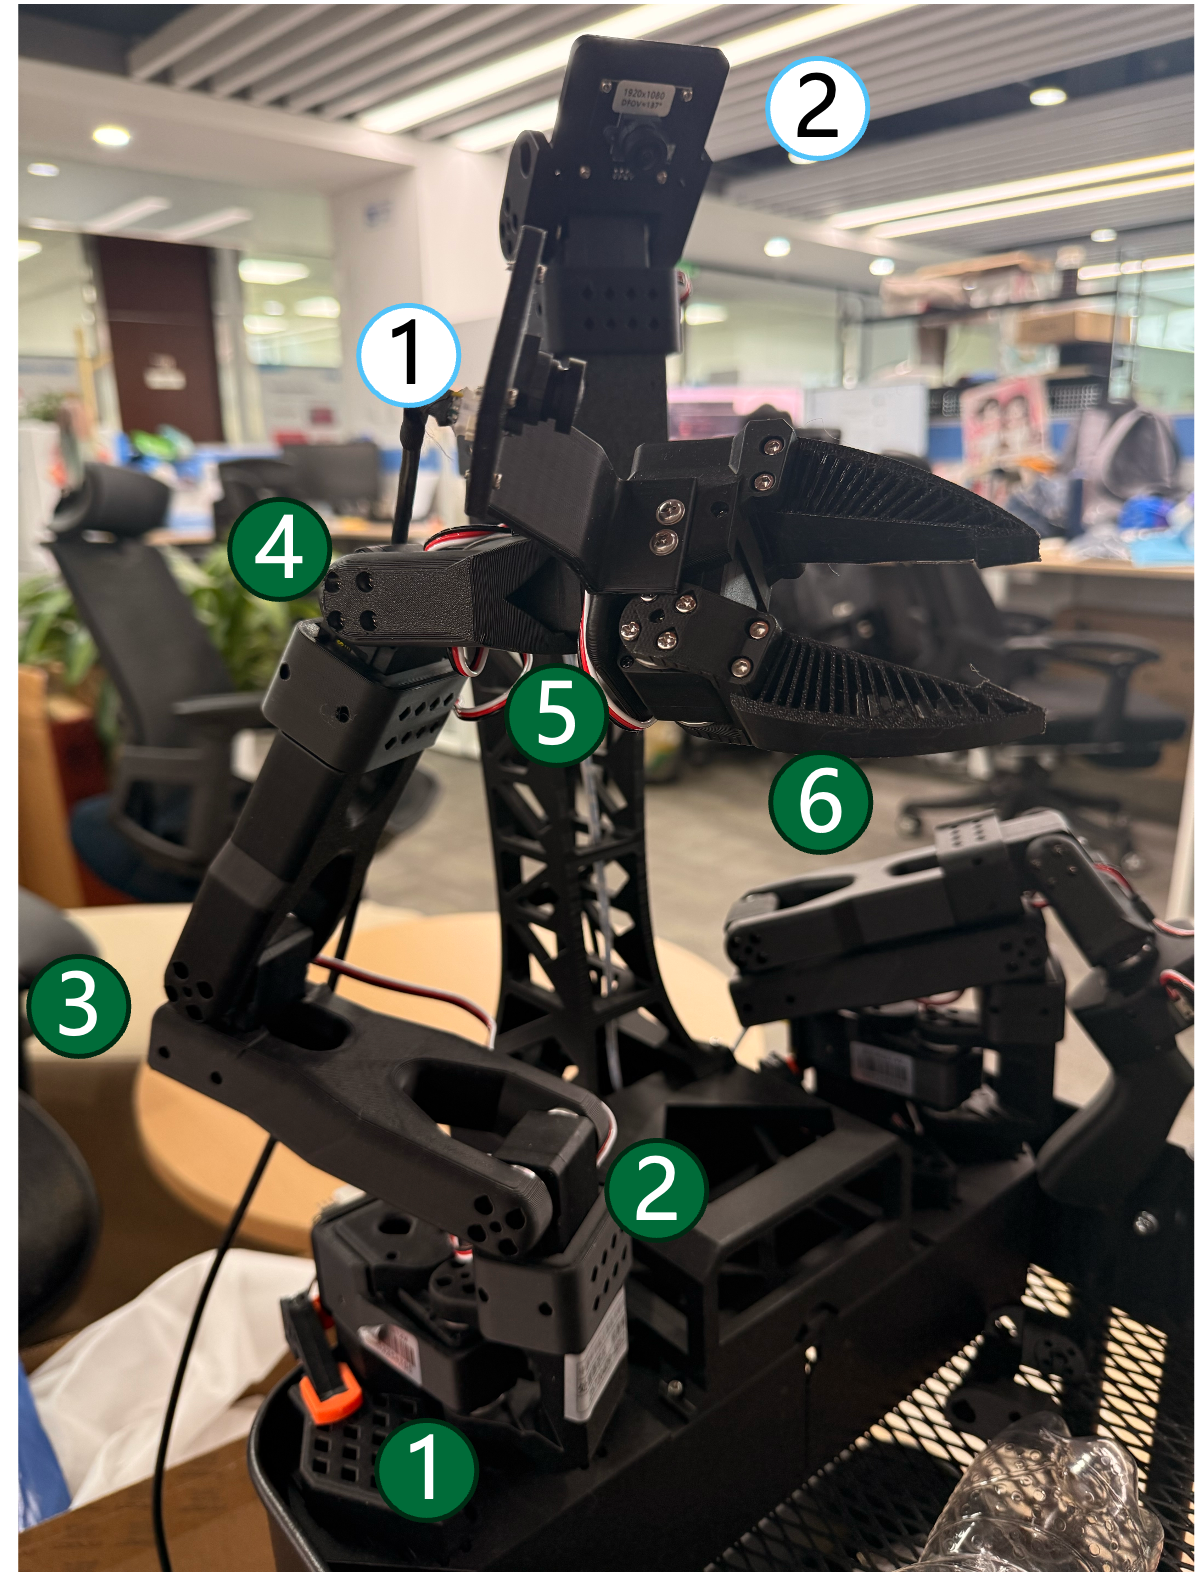
\includegraphics[width=0.55\textwidth]{2_实验环境构建/image/so101_hardware.png}
  \caption{SO-101 六自由度机械臂实物（标注关节编号 1--6）}
  \label{fig:so101-hardware}
\end{figure}

\begin{center}
\begin{tabular}{cll}
  \toprule
  编号 & 名称 & 说明 \\
  \midrule
  1 & shoulder\_pan  & 底座水平旋转关节 \\
  2 & shoulder\_lift & 肩部俯仰关节 \\
  3 & elbow\_flex    & 肘部弯曲关节 \\
  4 & wrist\_flex    & 腕部弯曲关节 \\
  5 & wrist\_roll    & 腕部滚转关节 \\
  6 & gripper        & 夹爪（末端执行器） \\
  \midrule
  C1 & handeye camera & 手眼相机，随臂运动，采集末端视角图像 \\
  C2 & fixed camera   & 固定相机，俯视工作台，采集场景全局图像 \\
  \bottomrule
\end{tabular}
\end{center}

策略模型选用 ACT\cite{act}（Action Chunking with Transformers），
以 ResNet18 + Transformer 构成约 50M 参数的端到端模仿学习策略。
以 RT-2\cite{rt2}、OpenVLA\cite{openvla} 为代表的 VLA 模型参数量达 7B+，
在无 GPU 的 ARM 平台上几乎无法实时运行；
Diffusion Policy\cite{diffusionpolicy} 参数量相近但扩散推理步数多导致延迟更高；
ACT 是本文研究场景下可在树莓派5 上实时运行的唯一可行选型。

\begin{center}
\begin{tabular}{p{0.22\textwidth}p{0.68\textwidth}}
  \toprule
  项目 & 配置 \\
  \midrule
  推理主机 & 树莓派5，ARM Cortex-A76，4 核，4 GB LPDDR4X，无 GPU \\
  机械臂 & SO-101 follower $\times 2$；推理时使用其中 1 个 follower \\
  舵机与驱动 & 每个 follower 含 6 个舵机，由 1 块舵机驱动板控制 \\
  摄像头 & USB 摄像头 $\times 2$，位置分别为 \texttt{handeye} 和 \texttt{fixed} \\
  图像采集 & OpenCV Camera，分辨率 640$\times$360，30 fps \\
  控制参数 & \texttt{chunk\_size=100}，控制目标 fps=30，串口波特率 1 Mbps \\
  采集设置 & 每类任务采集 $\geq 3$ 次 episode 取均值，排除冷启动影响 \\
  \bottomrule
\end{tabular}
\end{center}

\begin{center}
\begin{tabular}{p{0.22\textwidth}p{0.68\textwidth}}
  \toprule
  软件/库 & 版本或说明 \\
  \midrule
  操作系统 & Raspberry Pi OS \\
  Python & 3.10 \\
  LeRobot & 0.3.4 \\
  PyTorch & 2.7.1 \\
  torchvision & 0.22.1 \\
  OpenCV & 4.12.0.88 \\
  NumPy & 2.2.6 \\
  pyserial & 3.5 \\
  feetech-servo-sdk & 1.0.0 \\
  \bottomrule
\end{tabular}
\end{center}
